\newpage
\section{Comparison}
\begin{modified}
In order to compare two works, we decided to use the clustering \gls{fcm}, which is less sensitive to potential noise. This is particularly important in our case, as the comparison between two works leverages areas with lower densities, where noise could significantly affect the results.

\noindent In the previous study (\cite{thesis}), it was observed that the formula for comparing works was highly influenced by tiles with fewer occurrences. In our current context, which operates in a continuous space, these tiles correspond to regions with lower densities.

\noindent In this thesis, I developed an algorithm for comparing works and demonstrated its application through an example to better investigate its characteristics.
\end{modified}

\paragraph{Comparison value using KMeans}
\begin{modified} As already mentioned in \cref{chap:LiteratureReview}, we compared two works using their synthesized tiles. Specifically, we extracted two sets of tiles, $\mathcal{A},\mathcal{B}$, from the two works, where each tile is represented as a vector in $\mathbb{R}^K$. In \cite{thesis}, we employed predefined boxes to cluster the tiles. Each box had the same measure but contained a different number of data points (i.e., tiles). To analyze these clusters, we used a clustering algorithm, \gls{kmeans}, as described in \cref{chap:LiteratureReview}. Each cluster represents a region in the space $\mathbb{R}^K$ with its own measure and weights respect $\mathcal{A}, \mathcal{B}$.

\noindent The clustering procedure using \gls{kmeans} can be summarized as follows:
\begin{enumerate}
	\item Compute the \gls{kmeans} clustering of $\mathcal{L}:=\mathcal{A}\cup\mathcal{B}$. This gives the predictor $\mathcal{P}$, where $\mathcal{P}(x)$ is the centroid of the data point $x$.
	\item Compute the measure of each cluster: $\mu(C)=\sqrt{\mathbb{E}_{x\sim\mathcal{L}}\left[\left\|x-c\right\|^2\middle| \mathcal{P}(x)=c\right]}^K$ where $c$ is the centroid of the cluster.
	\item Compute the weight of each cluster with respect to $\mathcal{A}$: $p_\mathcal{A}(C)=\mathbb{P}_{x\sim\mathcal{A}}\left[\mathcal{P}(x)=c\right]$
	\item Compute the weight of each cluster with respect to $\mathcal{B}$: $p_\mathcal{B}(C)=\mathbb{P}_{x\sim\mathcal{B}}\left[\mathcal{P}(x)=c\right]$
	\item Compute the Jaccard Index:
	\begin{align*}
		D_\mathcal{A} &:= \texttt{clusters containing tiles from $\mathcal{A}$}\\
		D_\mathcal{B} &:= \texttt{clusters containing tiles from $\mathcal{B}$}\\
		\left|D_\mathcal{A}\cup D_\mathcal{B}\right| &= M \quad \texttt{(total number of clusters)} \\
		\left|D_\mathcal{A}\cap D_\mathcal{B}\right| &= \texttt{clusters containing tiles from both $\mathcal{A}$ and $\mathcal{B}$} \\
		J_{\mathcal{A},\mathcal{B}} &:= \frac{\left|D_\mathcal{A}\cap D_\mathcal{B}\right|}{\left|D_\mathcal{A}\cup D_\mathcal{B}\right|}
	\end{align*}
	\item Compute the measure of all clusters: $\mu(D_\mathcal{A}\cup D_\mathcal{B}) = \sum_{C\in D_\mathcal{A}\cup D_\mathcal{B}} \mu(C)$
	\item Compute the comparison value between the two works:
	\[
		d_{\gls{kmeans}}(\mathcal{A},\mathcal{B}) = \left(1+J_{\mathcal{A},\mathcal{B}}\right)^{-1}\frac{1}{\mu(D_\mathcal{A}\cup D_\mathcal{B})}\sum_C \mu(C)\left(\frac{p_\mathcal{A}(C)-p_\mathcal{B}(C)}{p_\mathcal{A}(C)+p_\mathcal{B}(C)}\right)^2
	\]
\end{enumerate}
\end{modified}

\subsection{Comparison value using FCM}
\begin{modified}
\noindent Next, we will apply \gls{fcm} to the fused distribution $\mathcal{L}$. Using fuzzy clustering, each data point will be assigned a degree of membership to multiple clusters, allowing for a more flexible representation of the data. For each cluster $C$ with centroid $c$, we will compute its size $\mu(C)$ and the weights of the set of samples, $p_\mathcal{A}(C)$ and $p_\mathcal{B}(C)$. Finally, we will redefine the Jaccard index between $D_\mathcal{A}$ and $D_\mathcal{B}$ within a fuzzy logic framework to better capture the similarities between the two sets.

\noindent The fuzzy nature of \gls{fcm} requires a redefinition of the cluster measure. Unlike \gls{kmeans}, where each data point is assigned to a single cluster by the predictor $\mathcal{P}$, in \gls{fcm} each data point has a degree of membership in multiple clusters. To extend the concept of cluster size, we define the measure of a cluster as a quantity proportional to the $K$ dimensional hypervolume of a hypersphere with radius equal to the mean square distance of the data from its centroid. For \gls{kmeans} this is expressed as:
\begin{equation*}
	\mu(C) = {\sqrt{\mathbb{E}_{x\sim\mathcal{L}}\left[\left\|x-c\right\|^2\middle|\mathcal{P}(x)=c\right]}\,}^{K} = {\sqrt{\frac{1}{\left|\{x\middle|\mathcal{P}(x)=c\}\right|}\sum_{x:\mathcal{P}(x)=c}\left\|x-c\right\|^2}\,}^{K}
\end{equation*}

\noindent In \gls{kmeans}, the algorithm aims to minimise the loss function:
\[
	\sum_{C\in\mathcal{C}}\sum_{x:\mathcal{P}(x)=c}\left\|x-c\right\|^2
\]
We get a different perspective of this loss function:
\begin{align*}
	\sum_{C\in\mathcal{C}}\sum_{x:\mathcal{P}(x)=c}\left\|x-c\right\|^2 &= \sum_{C\in\mathcal{C}}\left|\{x:\mathcal{P}(x)=c\}\right|\frac{1}{\left|\{x:\mathcal{P}(x)=c\}\right|}\sum_{x:\mathcal{P}(x)=c}\left\|x-c\right\|^2 \\
	&= N\sum_{C\in\mathcal{C}}\frac{\left|\{x:\mathcal{P}(x)=c\}\right|}{N}\mathbb{E}_{x\sim\mathcal{L}}\left[\left\|x-c\right\|^2\middle|\mathcal{P}(x)=c\right] \\
	&= N\sum_{C\in\mathcal{C}}\mathbb{P}_{x\sim\mathcal{L}}\left[\mathcal{P}(x)=c\right]\mathbb{E}_{x\sim\mathcal{L}}\left[\left\|x-c\right\|^2\middle|\mathcal{P}(x)=c\right] \\
	&= N\sum_{C\in\mathcal{C}} p(C)E(C)
\end{align*}
where $p(C):= \mathbb{P}_{x\sim\mathcal{L}}\left[\mathcal{P}(x)=c\right]$ and $E(C):= \mathbb{E}_{x\sim\mathcal{L}}\left[\left\|x-c\right\|^2\middle|\mathcal{P}(x)=c\right]$

\bigskip\noindent Extending this idea, we generalize the concept using the objective function of \gls{fcm}, as defined in \cref{def:fuzzyloss}. This allows the introduction of fuzzy membership.
\newpage
\begin{definition}[cluster's values]
\label{def:cluster_values}
	Applying \gls{fcm} to the data set $\mathcal{S}$ with weights $w$ and tiles in $\mathbb{R}^K$, we obtain the clusters $\mathcal{C}$ and the memberships $\mathds{1}$.

	\noindent We call the representability of cluster $C$ respect all other clusters the value: \\$p(C) = \frac{\sum_x w_x\mathds{1}_C(x)}{\sum_x w_x}$

	\noindent We call the concentration of cluster $C$ respect the membership measure the value: $\sigma(C) = \frac{\sum_x w_x\mathds{1}_C(x)^2}{\sum_x w_x\mathds{1}_C(x)}$
	\begin{remark}
		$\sigma(C)\in\left(0,1\right]$ because $\mathds{1}_C(x)\leq1$ and so: $\sum_x w_x\mathds{1}_C(x)^2 \leq \sum_x w_x\mathds{1}_C(x)$
	\end{remark}

	\noindent We call the mean square radius of the cluster $C$ with centroid $c$ the value: \\$E(C) = \frac{\sum_x w_x\mathds{1}_C(x)^2\left\|x-c\right\|^2}{\sum_x w_x\mathds{1}_C(x)^2}$

	\noindent The loss function of algorithm \gls{fcm} is can rewritted as:
	\[
		\mathcal{L}_\mathcal{S}(\mathcal{C}) = \left(\sum_x w_x\right)\sum_C p(C)\sigma(C)E(C)
	\]

	\noindent We denote by $\mu(c)$ the measure of the cluster $C$ with centroid $c$ as:
	\begin{equation}
		\label{def:cluster_measure}
		\mu(C) = \sigma(C)E(C)^{K/2} = \frac{\sum_x w_x\mathds{1}_C(x)^2}{\sum_x w_x\mathds{1}_C(x)}{\sqrt{\frac{\sum_{x\in\mathcal{S}} w_x\mathds{1}_C(x)^2 \left\|x-c\right\|^2}{\sum_{x\in\mathcal{S}}w_x\mathds{1}_C(x)^2}}\,}^K
	\end{equation}
\end{definition}
\end{modified}

\bigskip \noindent Similarly, we can define the values of the sets of tiles on the centroids:
\begin{toReview}
\begin{definition}
	\label{def:weightovercluster}
	Given a merged data set $\mathcal{S}=\mathcal{A}+\mathcal{B}$, where tiles belong in $\mathbb{R}^K$, and weights $w_\mathcal{A}$ and $w_\mathcal{B}$, the application of \gls{fcm} yields the set of clusters $\mathcal{C}$ and the membership degrees $\mathds{1}$ for each data point $x\in\mathcal{S}$.

	\noindent The representability of the set $\mathcal{A}$ with respect to a cluster $C$ is defined as
	$$ p_\mathcal{A}(C) = \frac{\sum_{x\in\mathcal{A}} w_x\mathds{1}_C(x)}{\sum_{x\in\mathcal{A}} w_x} $$

	\noindent Similarly, the representability of the set $\mathcal{B}$ with respect to a cluster $C$ is defined as
	$$ p_\mathcal{B}(C) = \frac{\sum_{x\in\mathcal{B}} w_x\mathds{1}_C(x)}{\sum_{x\in\mathcal{B}} w_x} $$
\end{definition}

\noindent In this way, we have defined both the cluster measures and the weights of each cluster for the sets of tiles $\mathcal{A}$ and $\mathcal{B}$. This completes part of the comparison formula, leaving the inclusion of the Jaccard index $J_{D_\mathcal{A},D_\mathcal{B}}$ as the next step:
\[
	\frac{1}{\mu(D_\mathcal{A} \cup D_\mathcal{B})} \sum_C \mu(C) \left(\frac{p_\mathcal{A}(C) - p_\mathcal{B}(C)}{p_\mathcal{A}(C) + p_\mathcal{B}(C)}\right)^2
\]
\end{toReview}

\paragraph{Fuzzy logic and the Jaccard Index}
\begin{toReview}
\noindent Defining the Jaccard index in fuzzy logic is a non-trivial task because the cardinality of a set is not defined in the same way as in Boolean logic. Unlike Boolean logic, where membership has a binary truth value (true or false), in fuzzy logic, membership degrees are continuous.

\noindent Even if \gls{fcm} is requested to produce $M$ centroids, not all clusters necessarily "exist". In Boolean logic, a cluster exists if at least one data point belongs to it. In fuzzy logic, however, no data point fully belongs to a specific cluster, and a data point can belong to multiple clusters simultaneously to varying degrees. Thus, the truth value of the statement "\texttt{$x$ belongs to the cluster $C$}" is $\mathds{1}_C(x)$. Extending this concept, the truth value of the existence of a cluster $C$ must also be defined. While there is no unique answer, we seek an acceptable and consistent definition for this operation.

\noindent Let $D_\mathcal{A}$ denote the set of clusters containing at least one data point from $\mathcal{A}$, and $\mathds{1}_{D_\mathcal{A}}(C)$ represent the degree to which the cluster $C$ exists within $D_\mathcal{A}$. Similarly, $\left|D_\mathcal{A}\right|$ represents the cardinality of the set of clusters, but in fuzzy logic, this cardinality is not an integer and can take continuous values. Below, we provide formal definitions for these concepts.

\begin{definition}(Jaccard index)
	\label{def:Jaccard_fcm}
	In fuzzy logic, the truth value of a logical disjunction is defined as the maximum of the truth values of its individual propositions. Based on this, the degree to which the cluster $C$ exists in $D_\mathcal{A}$ is given by:
	$$\mathds{1}_{D_\mathcal{A}}(C) = \max_{x\in\mathcal{A}}\mathds{1}_C(x)$$

	\noindent The cardinality of a set is defined as the sum of the membership degrees of all data points to the set. Thus, the cardinality of $D_\mathcal{A}$ is:
	$$|D_\mathcal{A}| = \sum_C \mathds{1}_{D_\mathcal{A}}(C)$$

	\noindent Consequently, the cardinality of the union of $D_\mathcal{A}$ and $D_\mathcal{B}$ is:
	$$|D_\mathcal{A} \cup D_\mathcal{B}| = \sum_c \mathds{1}_{D_\mathcal{A} \cup D_\mathcal{B}}(C) = \sum_C \max\{\mathds{1}_{D_\mathcal{A}}(C), \mathds{1}_{D_\mathcal{B}}(C)\} $$

	\noindent Similarly, the cardinality of the intersection of $D_\mathcal{A}$ and $D_\mathcal{B}$ is derived from the logical conjunction, which uses the minimum:
	$$|D_\mathcal{A} \cap D_\mathcal{B}| = \sum_C \mathds{1}_{D_\mathcal{A} \cap D_\mathcal{B}}(C) = \sum_C \min\{\mathds{1}_{D_\mathcal{A}}(C), \mathds{1}_{D_\mathcal{B}}(C)\} $$

	\noindent Based on these definitions, the Jaccard index for fuzzy logic is given by:
	\begin{equation*}
		J_{D_\mathcal{A},D_\mathcal{B}} :=
		\frac{
			\left|D_\mathcal{A} \cap D_\mathcal{B}\right|
		}{
			\left|D_\mathcal{A} \cup D_\mathcal{B}\right|
		}
		= \frac{
			\sum_C \min \left\{
				\max_{x\in \mathcal{A}}\left(
					\mathds{1}_{C}(x)
				\right), \max_{x\in \mathcal{B}}\left(
					\mathds{1}_{C}(x)
				\right)
			\right\}
		}{
			\sum_C \max\left\{
				\max_{x\in \mathcal{A}}\left(
					\mathds{1}_{C}(x)
				\right),\max_{x\in \mathcal{B}}\left(
					\mathds{1}_{C}(x)
				\right)
			\right\}
		}
	\end{equation*}
\end{definition}
\end{toReview}

\noindent The definitions provided in \cref{def:weightovercluster,def:cluster_measure,def:Jaccard_fcm} are sufficient to formulate the distance between two proposed samplings based on \gls{fcm}:
\[
d_{\text{\gls{fcm}}}\left(\mathcal{A},\mathcal{B}\right) = \left(1+J_{D_\mathcal{A},D_\mathcal{B}}\right)^{-1}\frac{1}{\mu(D_\mathcal{A} \cup D_\mathcal{B})} \sum_C \mu(C) \left(\frac{p_\mathcal{A}(C) - p_\mathcal{B}(C)}{p_\mathcal{A}(C) + p_\mathcal{B}(C)}\right)^2
\]

\subsection{Algorithm}
The algorithm initially involves applying \gls{fcm} to the fused dataset of the two works, in order to define the size and discretisation of the space of the tiles.
\begin{itemize}
	\item $ \mu(C) = \frac{\sum_x w_x\mathds{1}_{C}(x)^2}{\sum_x w_x\mathds{1}_C(x)}\sqrt{\frac{\sum_{x\in\mathcal{S}} w_x\mathds{1}_C(x)^2 \|x-c\|^2}{\sum_{x\in\mathcal{S}}w_x \mathds{1}_C(x)^2}\,}^K $
	\item $ p_\mathcal{A}(C) = \frac{\sum_{x\in \mathcal{A}} w_x\mathds{1}_C(x)}{\sum_{x\in \mathcal{A}}w_x} $ and similarly $ p_\mathcal{B}(C) = \frac{\sum_{x\in \mathcal{B}} w_x\mathds{1}_C(x)}{\sum_{x\in \mathcal{B}}w_x} $
	\item $ J_{D_\mathcal{A}, D_\mathcal{B}} $ as in \cref{def:Jaccard_fcm}
\end{itemize}
The distance between works will be defined as:
\begin{equation}
\label{eq:fuzzy_distance}
	d_{\gls{fcm}}(\mathcal{A}, \mathcal{B}) = (1 + J_{D_\mathcal{A}, D_\mathcal{B}})^{-1}\frac{\sum_C  \mu(c)\left(\frac{p_\mathcal{A}(C)-p_\mathcal{B}(C)}{p_\mathcal{A}(C)+p_\mathcal{B}(C)}\right)^2}{\sum_C \mu(C)}
\end{equation}

\begin{modified}
\noindent A simple application for a synthetic dataset is shown below, where we compare three methods for clustering and comparing two distributions $\mathcal{A}$ and $\mathcal{B}$. The three methods are:
\begin{itemize}
	\item \textbf{Box-clustering}: the space is partitioned into fixed, predefined boxes.
	\item \textbf{KMeans}: the space is divided into circular clusters, where each cluster is defined by its centroid and radius.
	\item \textbf{FCM}: the space is divided into fuzzy circular clusters, where each data point has a degree of membership to multiple clusters.
\end{itemize}

\noindent To illustrate these approaches, we generate two synthetic datasets $\mathcal{A}$ and $\mathcal{B}$ in a two-dimensional space. Each dataset consists of $150$ data points randomly sampled from six Gaussian distributions, with the addition of uniform noise. We cluster the merged dataset into $4$ clusters using each of the three methods.

\noindent In \cref{fig:box_clustering}, we show the box-clustering method, where the space is divided into a grid of fixed-size boxes, and each box contains a certain number of points from $\mathcal{A}$ and $\mathcal{B}$. In \cref{fig:kmeans_clustering}, we apply \gls{kmeans}, where the clusters are represented as circular regions centered at their respective centroids. Finally, in \cref{fig:fcm_clustering}, we use \gls{fcm} to produce fuzzy clusters, where the degree of membership of each data point is visualized using a color map.

\newpage
\begin{figure}[H]
	\centering
	\begin{subfigure}{0.48\linewidth}
		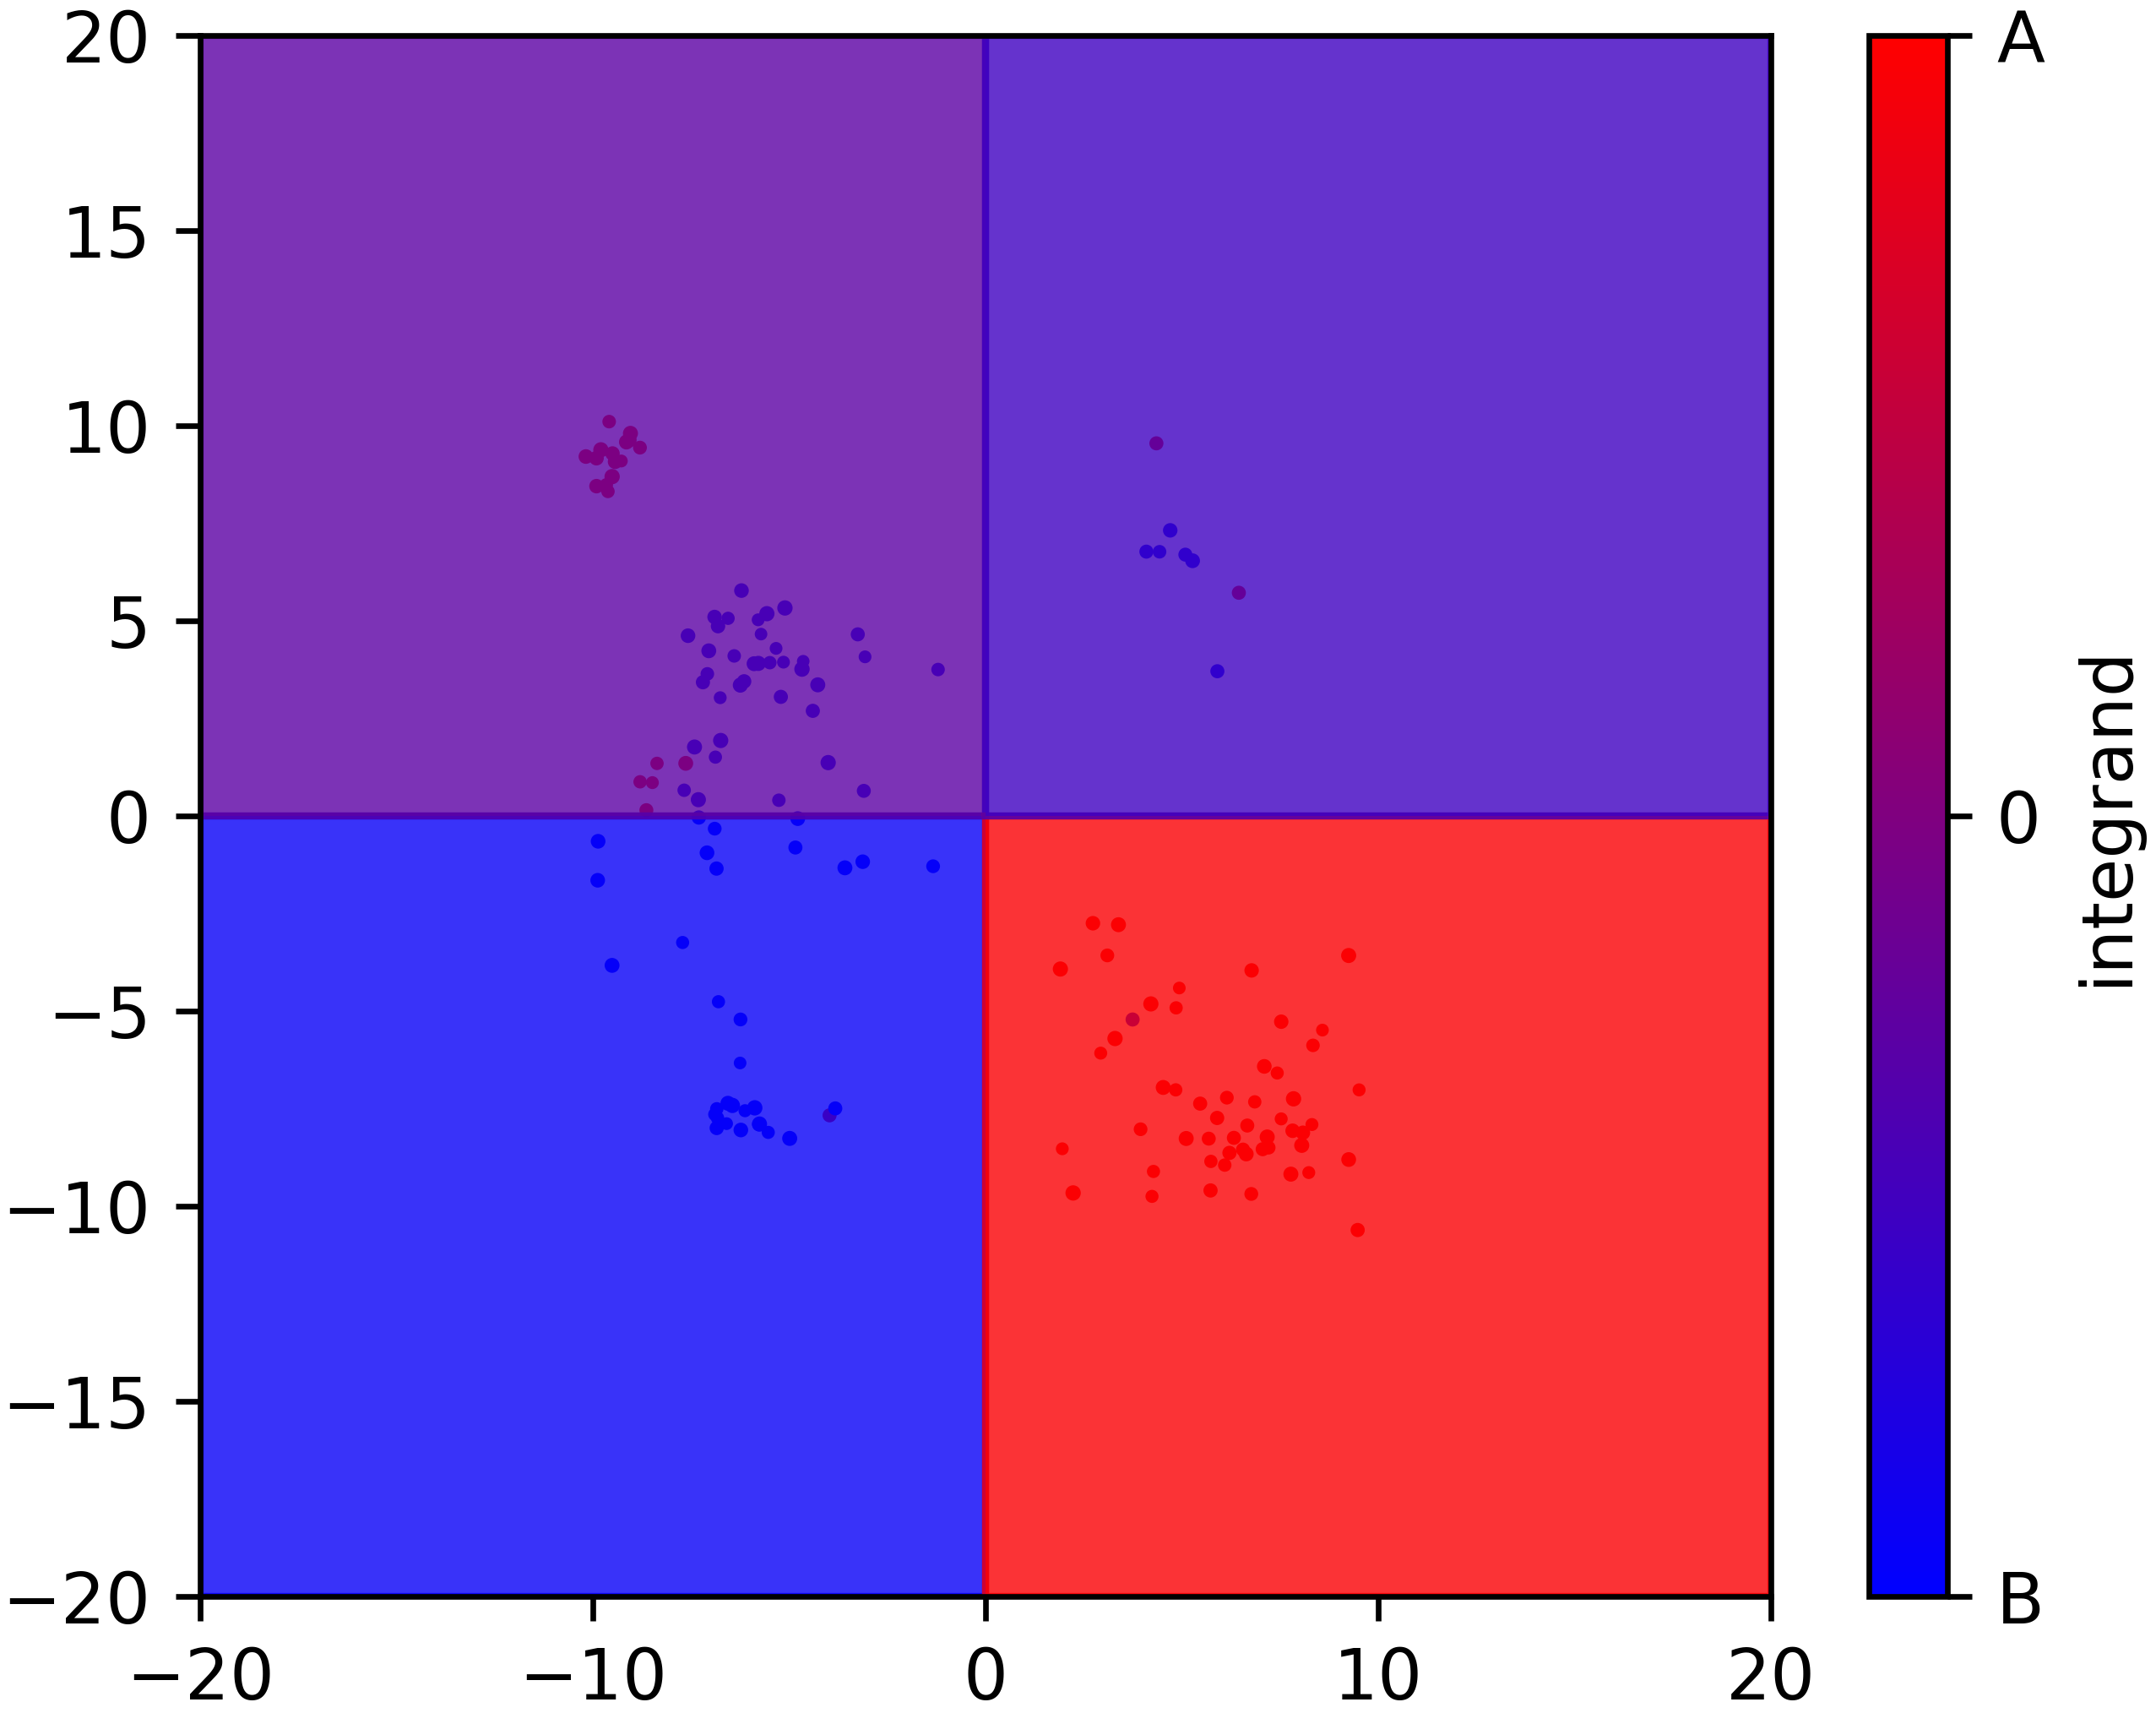
\includegraphics[width=\linewidth]{Figures/box_comparison.png}
		\caption[Box clustering, example of comparison]{Box clustering using $4$ boxes.\\ Computed distance: $0.268$.}
		\label{fig:box_clustering}
	\end{subfigure}
	\hfill
	\begin{subfigure}{0.48\linewidth}
		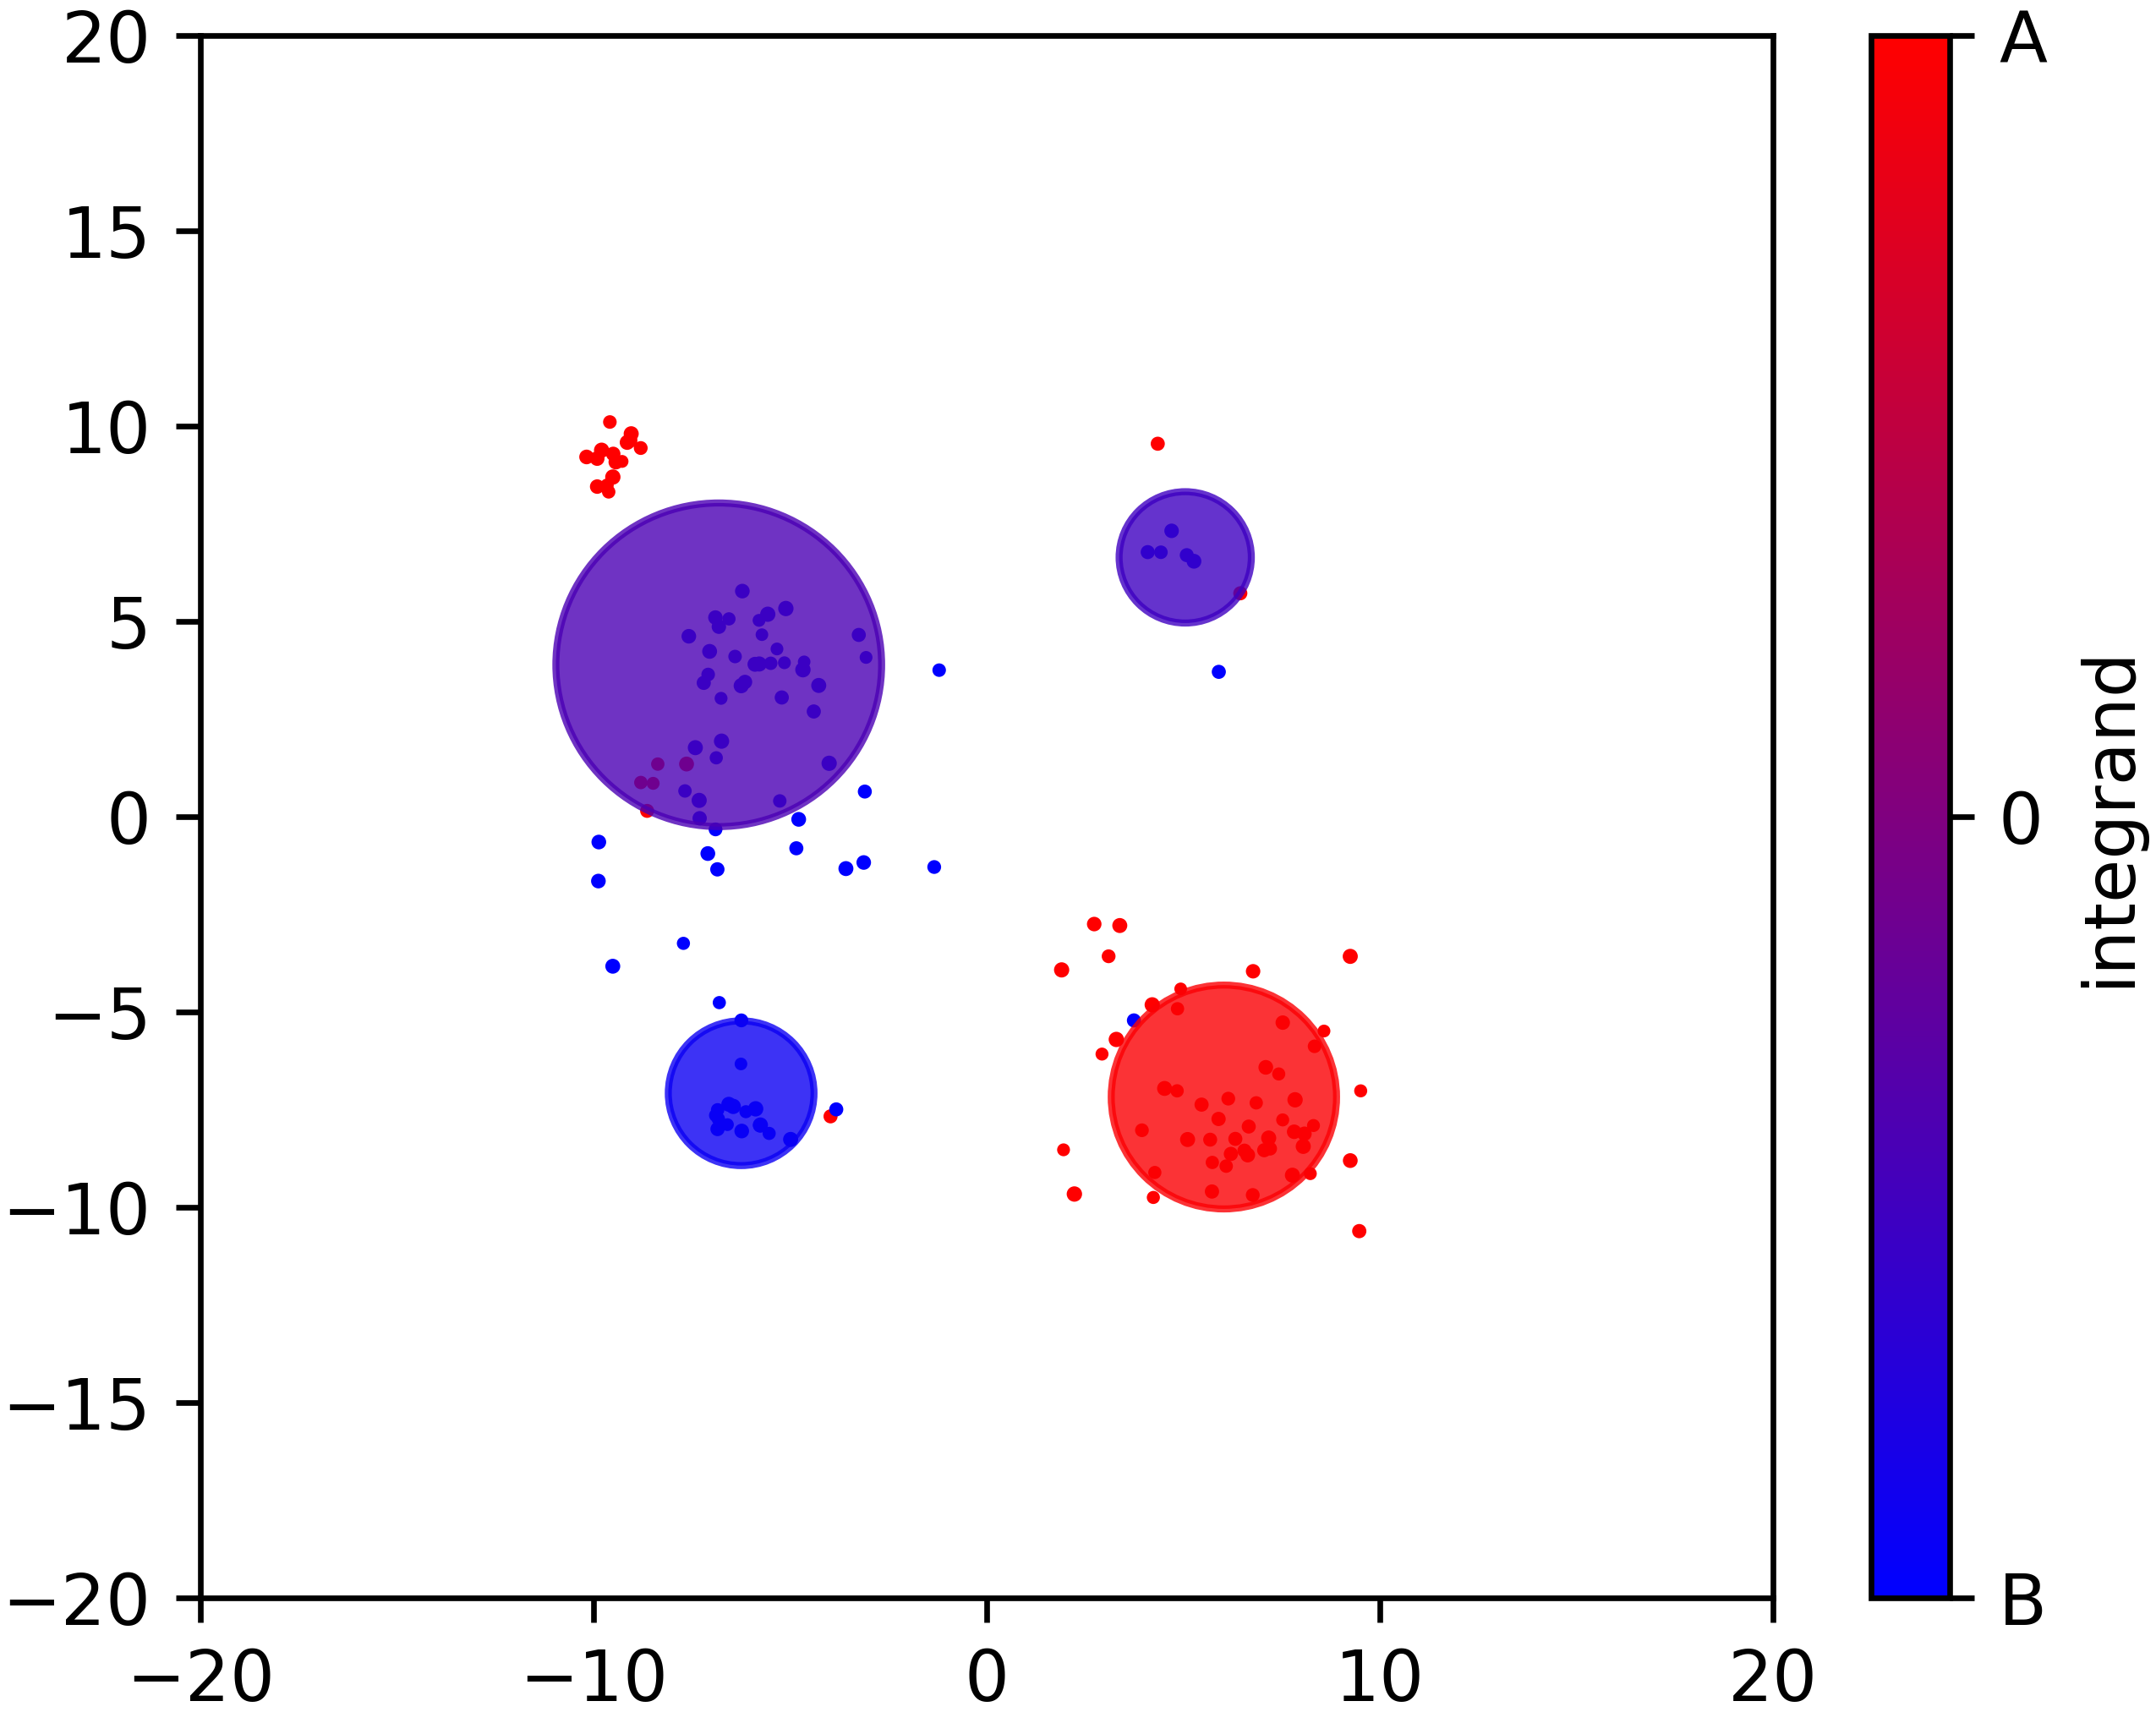
\includegraphics[width=\linewidth]{Figures/kmeans_comparison.png}
		\caption[\gls{kmeans} clustering, example of comparison]{\gls{kmeans} clustering using $4$ centroids.\\ Computed distance: $0.221$.}
		\label{fig:kmeans_clustering}
	\end{subfigure}
	\begin{subfigure}{\linewidth}
		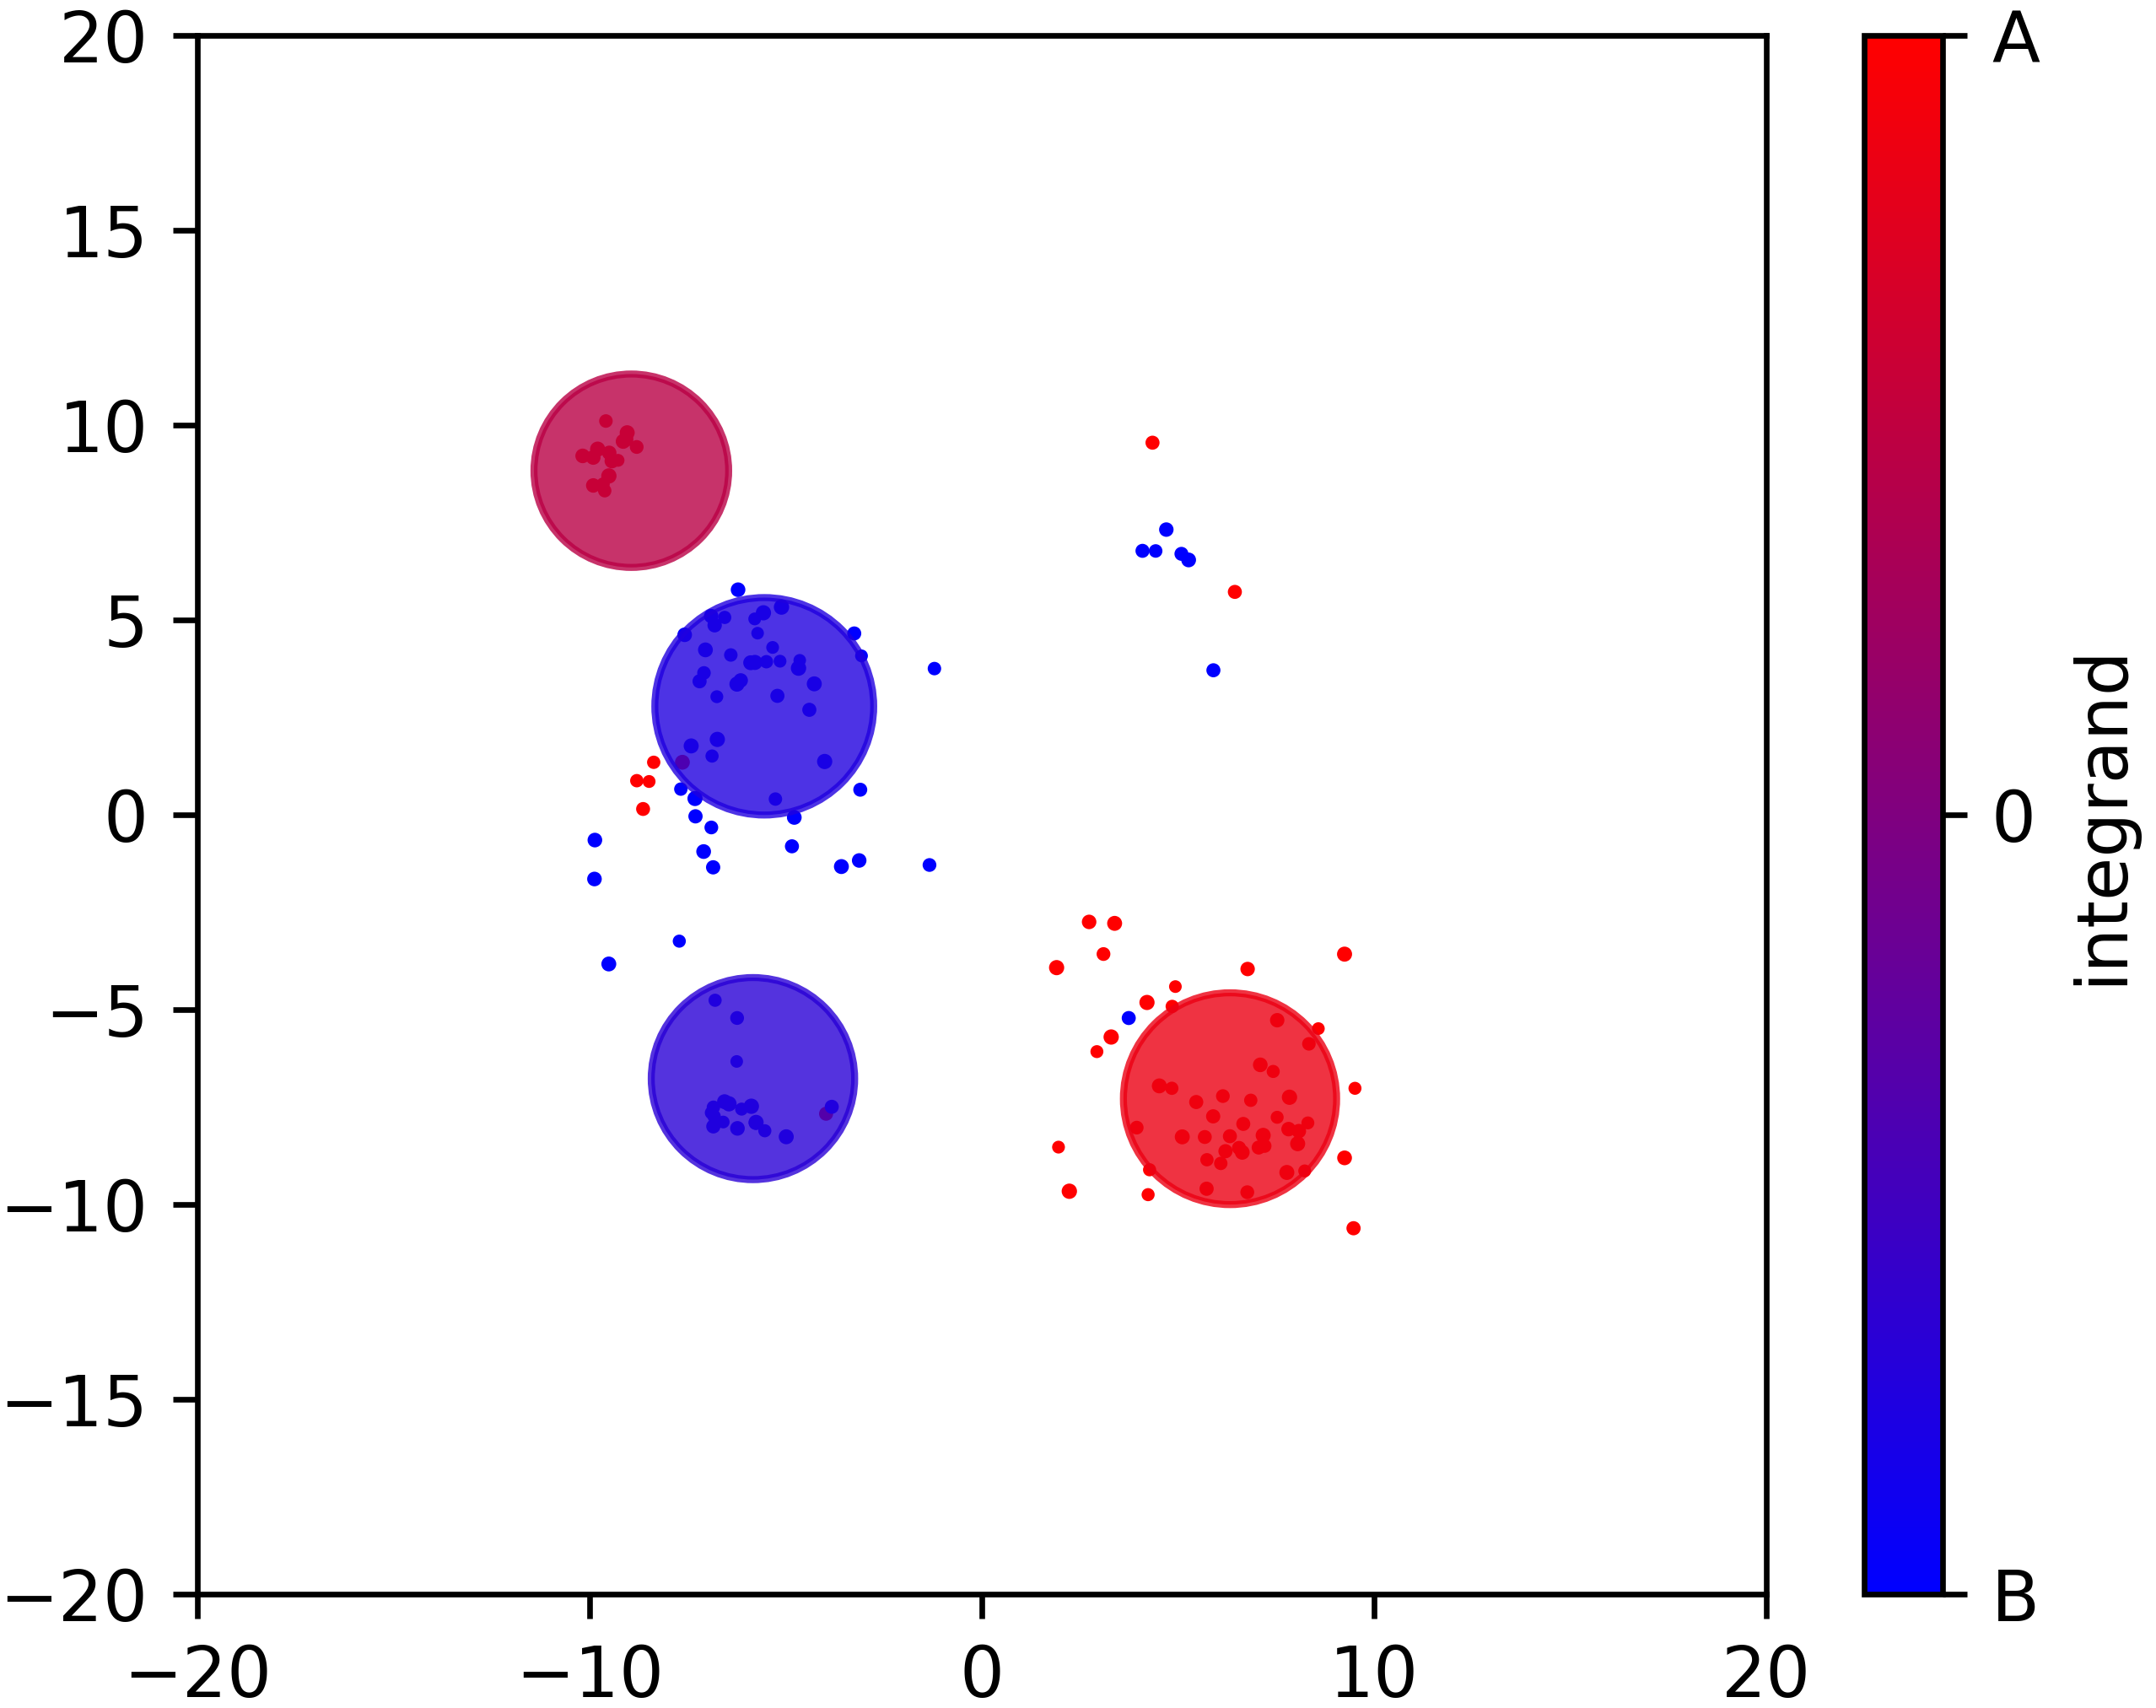
\includegraphics[width=\linewidth]{Figures/fcm_comparison.png}
		\caption[\gls{fcm} clustering, example of comparison]{\gls{fcm} clustering using $4$ centroids.\\ Computed distance $0.289$.}
		\label{fig:fcm_clustering}
	\end{subfigure}
	\caption[Comparing $3$ clustering techniques]{As can be seen, clusters are assigned a colour that is mapped to $[-1,1]$ ($-1$ is blue, $1$ is red). In particular, this colour is associated with the number $\frac{p_\mathcal{A}(C)-p_\mathcal{B}(C)}{p_\mathcal{A}(C)+p_\mathcal{B}(C)}$ for each cluster $C$. Furthermore, it is observed that \gls{kmeans} and \gls{fcm} have clusters represented by a circle with area $\mu(C)$ for the two clustering methods.}
\end{figure}
\end{modified}

\begin{modified}
\noindent In order to see the different perspective, we compare the different values obtained from box-clustering, \gls{kmeans} and \gls{fcm}.

\begin{table}[h]
	\centering
	\begin{tabular}{|>{\columncolor{pink}}c|c|c|c|}
		\hline
		\rowcolor{lavender}
		\cellcolor{mint} Values & Box-Clustering & \gls{kmeans} & \gls{fcm} \\
		$\left|D_\mathcal{A}\cap D_\mathcal{B}\right|$ & $4$ & $4$ & $2.889$ \\
		\hline
		$\left|D_\mathcal{A}\cup D_\mathcal{B}\right|$ & $4$ & $4$ & $3.980$ \\
		\hline
		$J_{D_\mathcal{A}, D_\mathcal{B}}$ & $1$ & $1$ & $0.7259$ \\
		\hline
		$\left(1+J_{D_\mathcal{A}, D_\mathcal{B}}\right)^{-1}$ & $0.5$ & $0.5$ & $0.5794$ \\
		\hline
		Integral & $0.5368$ & $0.4418$ & $0.4980$ \\
		\hline
		$d(\mathcal{A},\mathcal{B})$ & $0.268$ & $0.221$ & $0.289$ \\
		\hline
	\end{tabular}
	\caption[Comparison value using different clustering methods]{Comparing the values obtained from the $3$ algorithms, one can see how \gls{fcm} manages to provide a similar result using fuzzy logic.}
\end{table}
\end{modified}
\begin{toReview}
\begin{exempli_gratia}[Stability of \gls{fcm}]
	Consider a high-dimensional example comparing two sets of samples drawn from two Gaussian distributions with the gradual addition of uniform noise.

	\noindent The goal is to evaluate how noise affects the results obtained from \gls{fcm} compared to \gls{kmeans}.

	\noindent Specifically, we draw two sets of samples from the Gaussian distributions \(\mathcal{N}\left(-\vec{1}, \mathds{1}\right)\) and \(\mathcal{N}\left(\vec{1}, \mathds{1}\right)\) in \(\mathbb{R}^{16}\). Uniform noise with distribution \(\text{Unif}\left[-5, 5\right]^{16}\) is then added to the data.

	\noindent Each dataset consists of \(500\) samples, combining points from the Gaussian distributions and the noise. The table below shows how the distances between the two distributions decrease as the noise density increases.

	\begin{minipage}{\textwidth}
		\centering
		\begin{tabular}{|>{\columncolor{pink}}c|c|c|}
			\hline
			\rowcolor{lavender}
			\cellcolor{mint} Noise Density & \gls{kmeans} Distance & \gls{fcm} Distance \\
			$0\%$ & $1.000$ & $0.2975$ \\
			\hline
			$1\%$ & $0.5669$ & $0.2427$ \\
			\hline
			$2\%$ & $0.4858$ & $0.2411$ \\
			\hline
			$5\%$ & $0.4076$ & $0.2247$ \\
			\hline
			$10\%$ & $0.0491$ & $0.1921$ \\
			\hline
			$20\%$ & $0.0054$ & $0.1302$ \\
			\hline
		\end{tabular}
	\end{minipage}

	\noindent The results demonstrate that \gls{fcm} is significantly more robust than \gls{kmeans}, as it maintains a discernible distance between the two Gaussian distributions even in the presence of high noise density.
\end{exempli_gratia}
\end{toReview}

\paragraph{\gls{gpu}}
%L'algoritmo presentato è una soluzione sequenziale per l'estrazione delle tessere. Esso lavora iterando attraverso le righe e le colonne dell'immagine, estrae le tessere di dimensioni $N \times N$ e le inserisce in una lista. Tuttavia, questo approccio ha un costo computazionale pari a $O(hwN^2)$.\\
\noindent The \cref{alg:MembershipUpdateSafe} shown is a sequential solution for \gls{fcm}. It works by iterating through the data and centroids to compute the membership matrix. However, this approach has a computational cost of $O(NCK)$.

%Per migliorare l'efficienza computazionale, si può ricorrere all'utilizzo del boost della GPU (General Purpose Graphics Processing Unit). Questo genere di operazioni è noto come GPGPU (General-Purpose computing on Graphics Processing Units). Sfruttare la potenza di calcolo parallelo offerta dalle GPU può notevolmente accelerare il processo di estrazione delle tessere.
\noindent To improve computational efficiency, the use of \gls{gpu} \gls{boost}ing can be employed. This kind of operation is known as \gls{gpgpu}. Exploiting the parallel computing power offered by a \gls{gpu} can greatly accelerate the process of comparison.

%La \gls{gpu}, o unità di elaborazione grafica, è un componente elettronico presente in ogni computer, in grado di eseguire un grande numero di operazioni in parallelo. Originariamente concepita per gestire l'interfaccia grafica nei videogiochi, la \gls{gpu} si trova tipicamente nelle schede grafiche, dove è in grado di visualizzare miliardi di pixel sullo schermo di ogni computer a velocità che la \gls{cpu} non può raggiungere.\\
\noindent The \gls{gpu} is an electronic component present in every computer, able to perform a large number of operations in parallel. Originally designed to handle the graphical interface in video games, the \gls{gpu} is capable of handling billions of pixels on any computer screen at speeds that the \gls{cpu} cannot achieve.

%Questo processore è costituito da migliaia di thread, organizzati gerarchicamente a livello hardware per massimizzarne le prestazioni:
%\begin{enumerate}[label=\roman*.]
%\item \gls{sm}: Esegue un kernel e consiste di numerosi warp;
%\item \gls{warp}: Esegue il kernel del suo stream e possiede una memoria condivisa tra i suoi thread, di solito $32$;
%\item \gls{thread}: Esegue il kernel del suo warp sincronizzandosi con gli altri \gls{thread} dello stesso \gls{warp} e possiede una propria memoria riservata nei suoi registri.
%\end{enumerate}
\noindent This processor is made up of thousands of threads, organised hierarchically at the hardware level to maximise performance:
\begin{enumerate}[label=\roman*.]
\item \gls{sm}: Runs a kernel and consists of numerous \gls{warp}s;
\item \gls{warp}: Runs the kernel of its stream and has shared memory between its threads, usually $32$;
\item \gls{thread}: Executes the kernel of its warp by synchronising with the other \gls{thread}s of the same \gls{warp} and has its own reserved memory in its registers.
\end{enumerate}
%La memoria alla quale può accedere una \gls{gpu} è suddivisa in diverse categorie, tra cui la memoria \textit{global}, \textit{shared}, \textit{cache} e \textit{register}. L'accesso a queste memorie da parte dei \gls{thread} del processore dipende dalla gerarchia dei \gls{thread} stessi. Ad esempio, la memoria \textit{global} è accessibile da ogni \gls{thread}, mentre la memoria \textit{shared} è accessibile solo dai \gls{thread} appartenenti allo stesso \gls{warp}.\\
\noindent The memory that a \gls{gpu} can access is divided into different categories, namely \textit{global}, \textit{shared}, \textit{cache} and \textit{register} memory. Access to these memories by the processor's \gls{thread}s depends on the hierarchy of the \gls{thread}s themselves. For example, the \textit{global} memory is accessible by every \gls{thread}, while the \textit{shared} memory is only accessible by \gls{thread}s in the same \gls{warp}.

%In un computer di alta fascia, è comune trovare schede video dotate di $14$ \gls{sm}, ognuno dei quali contiene $1024$ \gls{thread} suddivisi in $32$ \gls{warp}. Questo totale di $14336$ \gls{thread} può eseguire in parallelo lo stesso identico codice, consentendo un'elaborazione estremamente veloce delle immagini e di altre operazioni che richiedono un alto grado di parallelismo.\\
\noindent In a high-end computer, it is common to find a \gls{gpu} with dozens of \gls{sm}, each containing $64$ or $128$ \gls{core}s. For example, if a process wants to use $\num{1024}$ threads on a single \gls{sm}, the \gls{gpu} will divide these threads into $32$ warps (each containing $32$ threads). Each warp is executed in chunks of $64$ threads at a time, meaning that $2$ warps can be executed simultaneously per clock cycle, while the remaining warps are scheduled for execution in subsequent cycles. This total of tens of thousands of \gls{thread}s can execute the exact same code in parallel, permitting extremely fast processing of images and other operations requiring a high degree of parallelism.

%A partire dagli anni $2000$, l'uso delle \gls{gpu} si è esteso al campo del calcolo scientifico, introducendo importati concetti come la scalabilità e l'\gls{hpc}. Dal $2020$, sono disponibili sul mercato \gls{gpu} dedicate alle operazioni di intelligenza artificiale.\\
\noindent Since the $2000$s, the use of \gls{gpu} has extended to the field of scientific computing, introducing important concepts such as scalability and \gls{hpc}. Since $2020$, dedicated \gls{gpu} are available on the market for artificial intelligence operations.

%In \gls{Python}, esistono framework utili per l'utilizzo delle \gls{gpu}, come \textit{torch} e \textit{TensorFlow}, ampiamente impiegati nell'ambito della computer vision. Tuttavia, anche linguaggi come il \verb"C++" offrono dialetti che consentono di sfruttare queste potenti unità di calcolo. In questo contesto, si userà il dialetto CUDA.\\
\noindent In \gls{Python}, there are useful frameworks for the utilisation of \gls{gpu}, such as \textit{torch} and \textit{TensorFlow}, which are widely employed in the field of computer vision. However, also languages such as \verb "C++" offer dialects that allow these powerful computing units to be exploited. In this paper, the \gls{cuda} dialect will be used.
\footnote{for more details about GPU architecture, see\newline\url{https://researchcomputing.princeton.edu/support/knowledge-base/gpu-computing}}
\footnote{for more details about \gls{cuda} language, see\newline\url{https://docs.nvidia.com/cuda/}}

\bigskip
\noindent The integration of \gls{gpgpu} techniques would allow the workload to be distributed over several cores of the \gls{gpu}, thus reducing the time needed for clustering operations. This method is particularly advantageous when handling large amounts of data, as the \gls{gpu} can perform many operations in parallel, speed up computation to be $2000$ times faster than the \gls{cpu} could have done.

\noindent The sum of $N$ numbers can be performed in with computational cost $O(log(N))$. This is because in parallel the \gls{gpu} threads sum one half of the vector over another at the same instant and then repeat until they get a single component that will have only one number. This operation is called \textit{reduction} and we can see it in the \cref{alg:gpu_reduction}. This is just one detail of how the \gls{gpu} can reduce the asymptotic computational cost of an algorithm. Suffice it to say that thanks to reductions and strong parallelism, it is possible to multiply two $N\times K$ and $K\times M$ matrices with cost $O(log(K))$ instead of $O(NMK)$. In clustering many operations can be parallelised and \gls{fcm} in particular requires many sums and linear operations.

\noindent The limitations of \gls{gpu} are not only related to the execution of the same operations on all threads, but also to the nature of these operations. Normally, an instruction takes much longer to be executed by a \gls{gpu} than by a \gls{cpu}. Arithmetic instructions are the most efficient, while the use of conditions tends to be avoided.

\begin{algorithm}
\caption[Parallel algorithm for sum reduction]{Parallel algorithm for sum reduction.\\
	\begin{minipage}[t]{\linewidth}
		\textsc{INPUT}
		\begin{itemize}[noitemsep, topsep=0pt]
			\item[$\textnormal{v}$:] array of values
			\item[$\textnormal{N}$:] number of components
		\end{itemize}
		This algorithm sum all values of an array and write in $\textnormal{v}[0]$ the result. The array is not preserved, in this way the algorithm does not allocate new memory. The computational cost is $O(\log(N))$. In \cref{fig:gpu_reduction} an example over a vector with $7$ components.
	\end{minipage}
}
\begin{algorithmic}[1]
\Procedure{Kernel $\textnormal{i}$, SumReduction}{$\textnormal{v}$,$\textnormal{N}$}
    \State Let $S$ a shared vector with $2^k \geq N$ component
    \State $S[\textnormal{i}] \gets \textnormal{v}[\textnormal{i}]$ if $\textnormal{i}<\textnormal{N}$ else $0$
    \For{$L \gets 2^{k}/2,2^{k}/4,\dots,1$}
        \If{$\textnormal{i} < L$}
            \State $S[\textnormal{i}] \gets S[\textnormal{i}] + S[\textnormal{i}+L]$
        \EndIf
        \State require synchronisation between threads
    \EndFor
\EndProcedure
\label{alg:gpu_reduction}
\end{algorithmic}
\end{algorithm}

\begin{figure}[h]
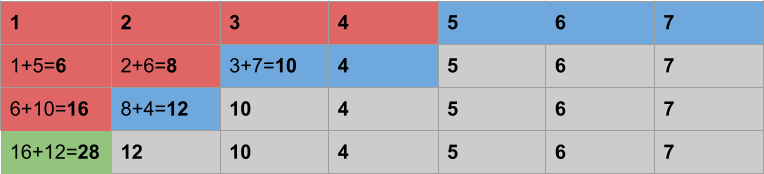
\includegraphics[width=\linewidth]{Figures/example_gpu_reduction.png}
\caption[Example of sum reduction performed by a GPU]{We want to calculate the sum of the values in the first row. The idea is to divide the vector into $2$ regions, sum the components, and repeat over the new vector with half the size of the previous vector.}
\label{fig:gpu_reduction}
\end{figure}
